%%%%%%%%%%%%%%%%%%%%%%%%%%%%%%%%%%%%%%%%%%%%%%%%%%%%%%%%%%%%%%%
%
% Welcome to writeLaTeX --- just edit your LaTeX on the left,
% and we'll compile it for you on the right. If you give
% someone the link to this page, they can edit at the same
% time. See the help menu above for more info. Enjoy!
%
%%%%%%%%%%%%%%%%%%%%%%%%%%%%%%%%%%%%%%%%%%%%%%%%%%%%%%%%%%%%%%%

% --------------------------------------------------------------
% This is all preamble stuff that you don't have to worry about.
% Head down to where it says "Start here"
% --------------------------------------------------------------
 
\documentclass[12pt]{article}
 
\usepackage[margin=1in]{geometry}
\usepackage{amsmath,amsthm,amssymb}

\usepackage{listings}
\usepackage{xcolor}
\usepackage{circuitikz}
\usetikzlibrary{bending}
\usetikzlibrary{patterns,decorations.pathmorphing,positioning}
\usepackage{enumitem}

\usepackage{tikz}
\usetikzlibrary{shapes,arrows,positioning,calc}
\tikzset{
block/.style = {draw, fill=white, rectangle, minimum height=3em, minimum width=3em},
tmp/.style  = {coordinate}, 
sum/.style= {draw, fill=white, circle, node distance=1cm},
input/.style = {coordinate},
output/.style= {coordinate},
pinstyle/.style = {pin edge={to-,thin,black}
}
}

\usepackage{float,graphicx}

%New colors defined below
\definecolor{codegreen}{rgb}{0,0.6,0}
\definecolor{codegray}{rgb}{0.5,0.5,0.5}
\definecolor{codepurple}{rgb}{0.58,0,0.82}
\definecolor{backcolour}{rgb}{0.95,0.95,0.92}

%Code listing style named "mystyle"
\lstdefinestyle{mystyle}{
  backgroundcolor=\color{backcolour}, commentstyle=\color{codegreen},
  keywordstyle=\color{magenta},
  numberstyle=\tiny\color{codegray},
  stringstyle=\color{codepurple},
  basicstyle=\ttfamily\footnotesize,
  breakatwhitespace=false,         
  breaklines=true,                 
  captionpos=b,                    
  keepspaces=true,                 
  numbers=left,                    
  numbersep=5pt,                  
  showspaces=false,                
  showstringspaces=false,
  showtabs=false,                  
  tabsize=2
}

%"mystyle" code listing set
\lstset{style=mystyle}

 
\newcommand{\N}{\mathbb{N}}
\newcommand{\Z}{\mathbb{Z}}
 
\newenvironment{theorem}[2][Theorem]{\begin{trivlist}
\item[\hskip \labelsep {\bfseries #1}\hskip \labelsep {\bfseries #2.}]}{\end{trivlist}}
\newenvironment{lemma}[2][Lemma]{\begin{trivlist}
\item[\hskip \labelsep {\bfseries #1}\hskip \labelsep {\bfseries #2.}]}{\end{trivlist}}
\newenvironment{exercise}[2][Exercise]{\begin{trivlist}
\item[\hskip \labelsep {\bfseries #1}\hskip \labelsep {\bfseries #2.}]}{\end{trivlist}}
\newenvironment{problem}[2][Problem]{\begin{trivlist}
\item[\hskip \labelsep {\bfseries #1}\hskip \labelsep {\bfseries #2.}]}{\end{trivlist}}
\newenvironment{question}[2][Question]{\begin{trivlist}
\item[\hskip \labelsep {\bfseries #1}\hskip \labelsep {\bfseries #2.}]}{\end{trivlist}}
\newenvironment{corollary}[2][Corollary]{\begin{trivlist}
\item[\hskip \labelsep {\bfseries #1}\hskip \labelsep {\bfseries #2.}]}{\end{trivlist}}

\newenvironment{solution}{\begin{proof}[Solution]}{\end{proof}}
 
\begin{document}
 
% --------------------------------------------------------------
%                         Start here
% --------------------------------------------------------------
 
\title{Homework 4}%replace X with the appropriate number
\author{Mengxiang Jiang\\ %replace with your name
EEEN 5338 Digital and DSP Based Control} %if necessary, replace with your course title
 
\maketitle
 
\begin{problem}{1} %You can use theorem, exercise, problem, or question here.  Modify x.yz to be whatever number you are proving
    For the following unity feedback system with
    $$G(s) = \frac{s+8}{s+5}$$
    which is digitally controlled with a sampling period of 0.02 seconds and a controller transfer function
    $$C(z) = \frac{0.35z}{z-1}$$.
    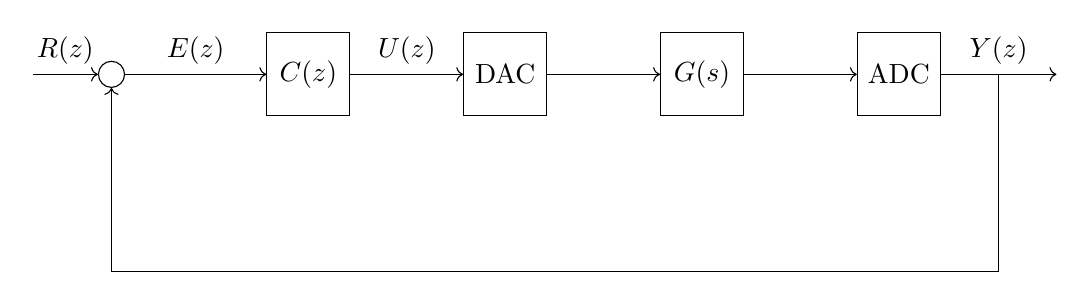
\begin{tikzpicture}[auto, node distance=2.5cm]
        \node [input, name=rin] (rin) {};
        \node [sum, right of=rin] (sum1) {};
        \node [block, right of=sum1] (c_z) {$C(z)$};
        \node [block, right of=c_z] (dac) {DAC};
        \node [block, right of=dac] (g_s) {$G(s)$};
        \node [block, right of=g_s] (adc) {ADC}; 
        \node [output, right of=adc, node distance=2cm] (output) {};
        \node [tmp, below of=sum1] (tmp1) {};
        \draw [->] (rin) -- node{$R(z)$} (sum1);
        \draw [->] (sum1) --node{$E(z)$} (c_z);
        \draw [->] (c_z) --node{$U(z)$} (dac);
        \draw [->] (dac) -- (g_s);
        \draw [->] (g_s) -- (adc);
        \draw [->] (adc) -- node [name=y] {$Y(z)$}(output);
        \draw [->] (y) |- (tmp1)-| (sum1);
        \end{tikzpicture}

    \begin{enumerate}[label=(\alph*)]
        \item Find the $z$-transfer function for the analog subsytem with DAC and ADC.
        \begin{align*}
            \frac{G(s)}{s} = \frac{s+8}{s(s+5)} = \frac{A}{s} + \frac{B}{s+5} \implies s+8 = (s+5)A + sB\\
            s = 0 \implies 8 = 5A \implies A = \frac{8}{5}=1.6\\
            s = -5 \implies 3 = -5B \implies B = -\frac{3}{5}=-0.6\\ 
            \implies \frac{G(s)}{s} = \frac{1.6}{s} - \frac{0.6}{s+5}\\
            G_{ZAS}(z) = (1-z{-1})\mathcal{Z}\left\{\frac{G(s)}{s}\right\}\\
            = \frac{z-1}{z}\left(\frac{1.6z}{z-1}-\frac{0.6z}{z-e^{-5(0.02)}}\right)\\
            = 1.6 - \frac{0.6(z-1)}{z-e^{-0.1}}\\
            \text{using Wolfram Alpha to simplify the algebra:}\\
            G_{ZAS}(z)= \frac{z-0.84774}{z-0.904837}
        \end{align*}
        \item Find the closed-loop transfer function and characteristic equation.\\\\
        transfer function:
        \begin{align*}
            G_{cl}(z) = \frac{C(z)G_{ZAS}(z)}{1+C(z)G_{ZAS}(z)}\\
            = \left(\frac{0.35z(z-0.84774)}{(z-1)(z-0.904837)}\right)/\left(1+\frac{0.35z(z-0.84774)}{(z-1)(z-0.904837)}\right)\\
            \text{using Wolfram Alpha to simplify the algebra:}\\
            G_{cl}(z)= \frac{0.259259(z-0.84774)z}{z^2-1.63077z + 0.67025}\\
        \end{align*}
        characteristic equation:
        \begin{align*}
            1+C(z)G_{ZAS}(z) = 0\\
            z^2-1.63077z + 0.67025 = 0
        \end{align*}
        \item Find the steady-state error due to a sampled unit step and a sampled unit ramp. Comment on the effect of the controller on steady-state error.
        \begin{align*}
            C(z)G_{ZAS}(z) = L(z)\\
            \implies L(z) = \frac{0.35z(z-0.84774)}{(z-1)(z-0.904837)}\\
            \implies \text{system is type 1}\\
        \end{align*}
        The steady state error for a sampled unit step is 0 for type 1 and higher.\\
        The steady state error for a sampled unit ramp is:
        \begin{align*}
            e(\infty) = \frac{T}{(z-1)L(z)|_{z=1}} = \frac{0.02}{\frac{0.35(1-0.84774)}{1-0.904837}} = 0.035714
        \end{align*}
        If the controller has additional pole(s) at unity, the type of the system can be increased to make the steady-state error 0 for the unit ramp.
    \end{enumerate}
\end{problem}
\pagebreak
\begin{problem}{2}
    Use MATLAB for the following system with a sampling period of 0.05 seconds:
    $$G(s) = \frac{10(s+2)}{s(s+5)}$$
    \begin{enumerate}[label=(\alph*)]
        \item Obtain the transfer function for the system with sampled input and output.
        \begin{figure}[H]
            \centering
            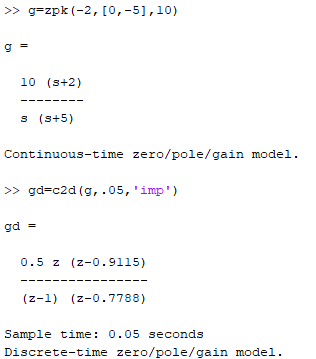
\includegraphics{2a}
        \end{figure}
        \item Obtain the transfer function for the system with DAC and ADC.
        \begin{figure}[H]
            \centering
            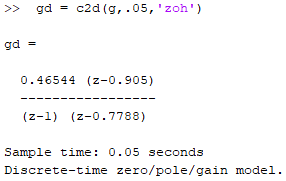
\includegraphics{2b}
        \end{figure}
        \pagebreak
        \item Obtain the unit step response of the system with sampled output and analog input.
        \begin{figure}[H]
            \centering
            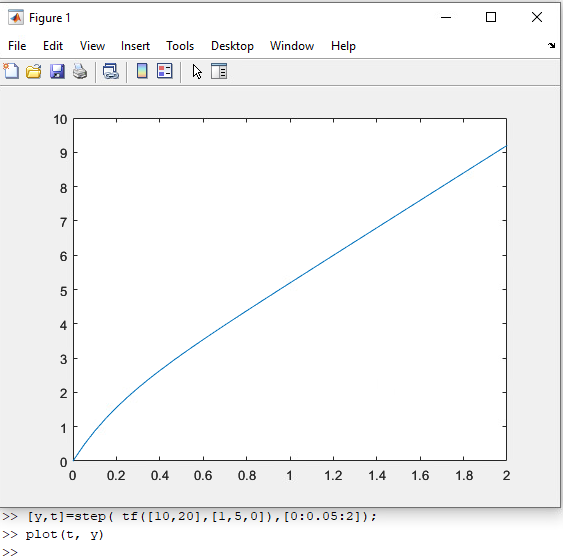
\includegraphics{2c}
        \end{figure}
        \item Obtain the poles of the system in (a), (b), and the output of (c) and comment on the differences between them.\\\\
        Both (a) and (b) have poles at 1 and 0.7788. (c) has an additional pole at 1 from the unit step.
    \end{enumerate}
\end{problem}

% --------------------------------------------------------------
%     You don't have to mess with anything below this line.
% --------------------------------------------------------------
 
\end{document}